

   \subsection{Sequence Diagram}

\hspace{5mm}Sequence diagrams shows the object interactions arranged in time sequence, describing how and in what order a group of objects works together.

In below, sequence diagram shows how the user should enter inputs when registering to the system. If the user enters valid input, the system redirects to the login page, and if the user enters invalid inputs, the system shows error messages.\newline

\begin{center}
    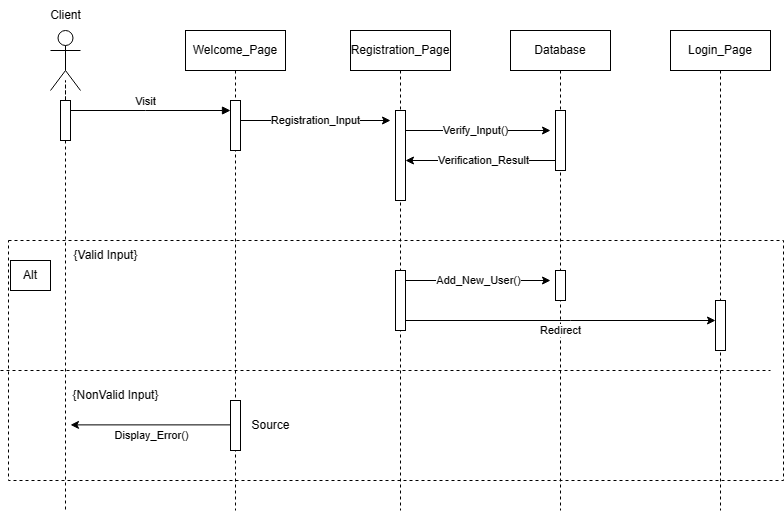
\includegraphics[scale=0.6]{SequenceDiagram_WelcomePageRegisterPage.png}
    \caption{Welcome Page and Registration Sequence Diagram}
\end{center}

In this sequence diagram, one can observe how login authentication works. As shown in the diagram, if the user enters valid  login credentials the system redirects to the Main Page, and if the user enters invalid login credential error is dispatch for to display.
    
\begin{center}
    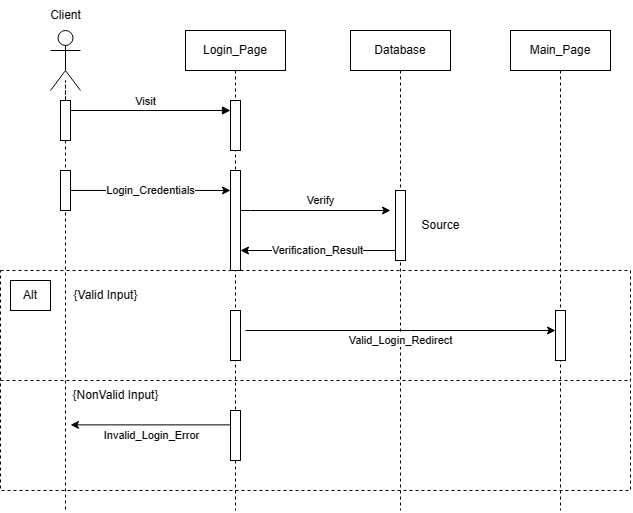
\includegraphics[scale = 0.8]{SequenceDiagram_LoginPage.png}
    \caption{Login page Sequence Diagram}
\end{center}

In this sequence diagram, one can observe how login authentication works. As shown in the diagram, if the user enters valid  login credentials the system redirects to the Main Page, and if the user enters invalid login credential error is dispatch for to display.

\begin{center}    
    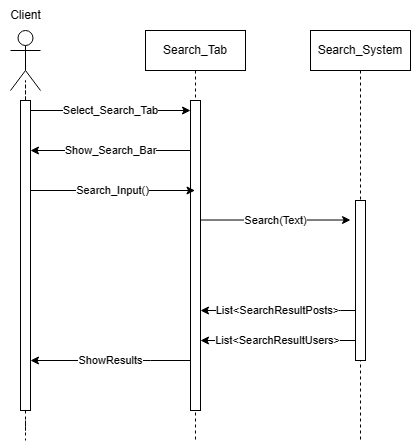
\includegraphics[scale = 1]{SequenceDiagram_SearchTab.png}\\
    \caption{Search Tab Sequence Diagram}
\end{center}

    In this sequence diagram, one can observe how search operation of the posts and users works. As shown in the diagram, user enters a keyword to the search bar. Search systems handles the requested keyword and returns if there exist any users or posts with that keyword. Then these lists will be shown to the user.

\begin{center} 
    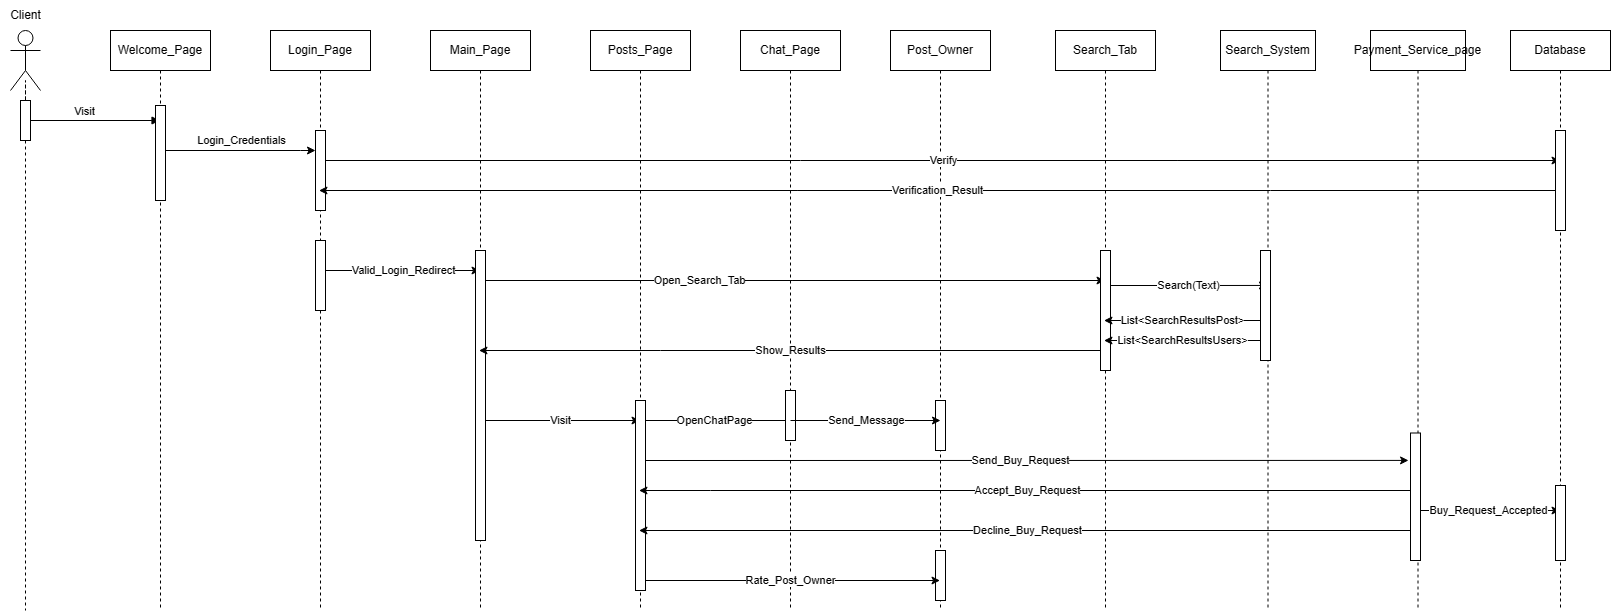
\includegraphics[scale = 0.3]{SequenceDiagram_Post.png}
    \caption{Post Sequence Diagram}
\end{center}

In this sequence diagram, one can observe a user interacts with the system from the perspective of post related operations. In each step, diagram shows which inputs we have obtained. By these response inputs we are showing how each post related operation is handled within the system and the resultant directions.
%describe here the sequence diagram